\section{Evidence accounting and scoped verification}
\label{sec:evidence}

The evidence layer separates a source's assertion, its archived representation,
and a subsequent assessment. Its concrete implementation is the
\code{EvidenceLedger} Python class, which stores versioned JSON records in
SQLite. The record names in Table~\ref{tab:evidence} identify dictionary
discriminators rather than seven corresponding Python classes. Analysis
functions separately exchange schema-validated JSON-compatible documents.
Their provenance relationships are conceptually related to PROV, without
demonstrated RDF export or PROV-O conformance
\citep{moreau2013provdm,lebo2013provo}.

\begin{table}[tb]
\centering
\small
\caption{Concrete ledger record kinds and enforced boundaries. Referential
integrity establishes traceability; it does not establish evidential entailment.}
\label{tab:evidence}
\begin{tabularx}{\linewidth}{@{}lXX@{}}
\toprule
Record kind & Stored content and links & Principal structural constraint \\
\midrule
Source & URI, title, publisher, publication time & Identifier and required metadata \\
Artifact & Source link, path, digest, capture time & Existing source; SHA-256 syntax \\
Passage & Artifact link, text, locator & Existing artifact; nonempty text \\
Claim & Statement, type, source/evidence links & Attributed source or finding evidence \\
ClaimMention & Claim and passage links & Published claim and same-source passage \\
EvidenceAssessment & Claim, status, evidence, rationale & Valid references and supersession chain \\
VerificationResult & Scope, cutoff, status, evidence sides & Status-consistent evidence references \\
\bottomrule
\end{tabularx}
\end{table}

The ledger rejects updates and deletions through SQLite triggers. Re-inserting
an identical record is idempotent; reusing its identifier with different content
fails. Assessments and verification results may supersede earlier records
without replacing them, and supersession must target the same claim and cannot
branch. An artifact's digest is format-checked rather than recomputed from the archived
file by the ledger itself. A passage locator may contain arbitrary JSON; exact
text-span checking belongs to the separate assessment constructor.
Figure~\ref{fig:provenance} illustrates these distinctions.

\begin{figure}[tb]
\centering
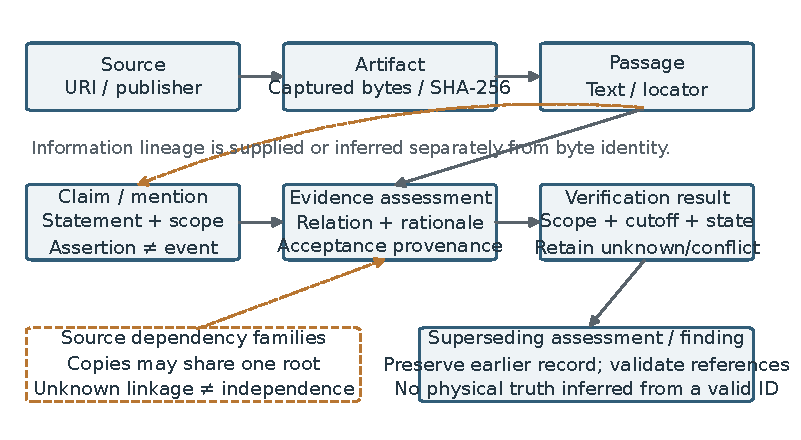
\includegraphics[width=\linewidth]{evidence_provenance.pdf}
\caption{Evidence and provenance relationships. Source assertions, artifact
bytes, extracted passages, and analytical judgments remain distinct. Recorded
lineage and valid locators support inspection without guaranteeing truth or
source independence.}
\label{fig:provenance}
\end{figure}

Local retrieval uses BM25 over supplied passages, searches claim and
counterevidence directions, and respects a capture-time cutoff and query budget.
Results remain unassessed candidates. An assessment constructor checks that its
quoted Unicode-codepoint span equals the passage substring, validates scope and
numeric constraints, and records acceptance provenance. Accepted assessments
require either a human-adjudication label or a validated-rule label with a rule
identifier. This is a structural requirement: the constructor does not consult
an independently validated rule registry. The dedicated claim builder supplies
the latter label programmatically.

The shared verification vocabulary contains seven states:
\code{unverified}, \code{supported_within_scope},
\code{refuted_within_scope}, \code{conflicting_evidence},
\code{insufficient_evidence}, \code{not_verifiable}, and \code{superseded}.
It excludes candidate-only, mistimed, scope-mismatched, or improperly cited
assessments. Verdict thresholds count declared source-lineage identifiers;
separate fields count roots explicitly marked independently confirmed.
These quantities must not be conflated. A physical-fact scope additionally
requires an accepted direct physical evidence basis before support or refutation
can stand. Institutional denials can therefore remain recorded as an official
position while the physical claim remains insufficiently evidenced. This guard
depends on the supplied scope type; it does not independently classify a claim's
epistemic scope.

The curated case package contains 25 claims, 25 selected passages, and 36 accepted
rule assessments. Its current schema~2.3 outputs are 19 supported, zero refuted,
and six insufficient-evidence results. These are program outputs, not accuracy
measurements. The earlier schema~2.0 package produced 21 supported and four
refuted results from 31 assessments, while injecting designated passages and
expected relations into assessment construction. Current code assesses only
retrieved candidates and removes that direct injection, but claims, queries,
passages, scopes, and lineage labels remain curated. The general offline runner
is more restricted: it retrieves candidates and creates no accepted assessments.

Two hand-designed challenges expose semantic failures in the current matcher.
A passage about 26 trees is accepted as supporting a claim about 26 military
occupants, and a sentence negating police arrival is accepted as supporting
arrival. Both receive the fixed branch confidence 0.92. The stored case artifact
also accepts injury and independent-walking passages as support for a claim about
four deserters. Numeric agreement can satisfy the support rule without matching
the predicate; lexical overlap can miss ordinary negation. Moreover, inference
uses the entire passage while the stored citation may be a shorter retrieved
span. Exact quotation therefore does not guarantee that the quotation entails
the assigned relation.

No independent local gold set establishes entailment accuracy or calibrates these
confidence values. The challenges demonstrate failures rather than estimating
their prevalence. FEVER and AVeriTeC motivate evaluating evidence adequacy jointly
with verdict correctness \citep{thorne2018fever,schlichtkrull2023averitec,
schlichtkrull2024averitec}; they provide no substitute for evaluating this system
on independently adjudicated claims. InFact provides an external staged comparator
\citep{rothermel2024infact}, not a measured baseline here.
